\section{Data and simulated samples}\label{sec:Dataset}

\subsection{2016 dataset}
%Data
Data recorded in proton proton collisions at 13~TeV during all 2016 was used in the analysis, with a total integrated luminosity of  35.9 \fbinv.
The data has been reprocessed in the reprocessing campaign characterized by the submission date \textit{03Feb2017}.
In Table~\ref{tab:data} the different data streams used are presented. All
runs are taken at 25~ns and recorded in seven different periods.
%
%\begin{table*}[htbH]
%\begin{center}
%\caption{Data samples used in the analysis. 
%\label{tab:data}}
%\begin{tabular}{@{}|l|c|c|@{}}
%\hline
%Data Taking Era & Stream & Luminosity\\
%\hline
%\multirow{5}{*}{Run2015D - 05 Oct 2015} 	& SingleMuon & \\
%								& SingleElectron & \\
%								& DoubleEG &  0.553~\ifb\\
%								& DoubleMuon & \\
%								& MuonEG & \\ \hline
%\multirow{5}{*}{Run2015D - PromptReco} 	& SingleMuon & \\
%								& SingleElectron & \\
%								& DoubleEG & 1.566~\ifb  \\
%								& DoubleMuon & \\
%								& MuonEG & \\ 								
%\hline 
%\end{tabular}
%\end{center}
%\end{table*}

\begin{table*}[htbH]
\begin{center}
\begin{tabular}{@{}|l|c|@{}}
\hline
Data Taking Era & Stream\\
\hline
\multirow{5}{*}{Run2016C} 	& SingleMuon  \\
                                & DoubleMuon \\
				& SingleElectron \\
                                & DoubleEG \\
				& MuonEG \\ \hline
\multirow{5}{*}{Run2016D}       & SingleMuon  \\
                                & DoubleMuon \\
                                & SingleElectron \\
                                & DoubleEG \\
                                & MuonEG \\ \hline
\multirow{5}{*}{Run2016E}       & SingleMuon  \\
                                & DoubleMuon \\
                                & SingleElectron \\
                                & DoubleEG \\
                                & MuonEG \\ \hline
\multirow{5}{*}{Run2016F}       & SingleMuon  \\
                                & DoubleMuon \\
                                & SingleElectron \\
                                & DoubleEG \\
                                & MuonEG \\ \hline
\multirow{5}{*}{Run2016G}       & SingleMuon  \\
                                & DoubleMuon \\
                                & SingleElectron \\
                                & DoubleEG \\
                                & MuonEG \\ \hline
\multirow{5}{*}{Run2016H}       & SingleMuon  \\
                                & DoubleMuon \\
                                & SingleElectron \\
                                & DoubleEG \\
                                & MuonEG \\ \hline
\hline 
\end{tabular}
\caption{Data samples used in the analysis. The total integrated luminosity
corresponds to 35.9\fbinv.
\label{tab:data}}
\end{center}
\end{table*}
%

The triggers used in the analysis are summarized in Table~\ref{tab:triggers} 

\begin{table}
\begin{center}
\begin{tabular}{|l|l|}
   \hline
   Dataset & HLT path \\
   \hline
   
   \multirow{2}{*}{SingleElectron} & HLT\_Ele45\_WPLoose\_Gsf\_v* \\
                                   & HLT\_Ele27\_eta2p1\_WPLoose\_Gsf\_v* \\
   \hline
   
   \multirow{2}{*}{SingleMuon}   & HLT\_IsoMu22\_v* \\
                                 & HLT\_IsoTkMu22\_v* \\
   \hline
   
   \multirow{2}{*}{MuonEG}       & HLT\_Mu8\_TrkIsoVVL\_Ele17\_CaloIdL\_TrackIdL\_IsoVL\_v*  \\
                                 & HLT\_Mu17\_TrkIsoVVL\_Ele12\_CaloIdL\_TrackIdL\_IsoVL\_v*  \\
   
   \hline
   
   \multirow{2}{*}{DoubleMuon}   & HLT\_Mu17\_TrkIsoVVL\_Mu8\_TrkIsoVVL\_v*  \\
                                 & HLT\_Mu17\_TrkIsoVVL\_TkMu8\_TrkIsoVVL\_v*  \\

   
   \hline
   
   \multirow{1}{*}{DoubleEG}   &    HLT\_Ele23\_Ele12\_CaloIdL\_TrackIdL\_IsoVL\_DZ\_v* \\
   
   \hline
\end{tabular}
\caption{
    HLT paths used in the analysis.
\label{tab:triggers}  }
\end{center}
\end{table}

In Figure~\ref{Fig:trigger} the trigger efficiency for a gluon fusion signal
with mass 300~\GeV is shown for electrons (left) and muons (right).
An average trigger efficiency greater than 99\% is found, as shown in Figure~\ref{Fig:triggerIntegral}.


\begin{figure*}[htbp]
\centering
\begin{tabular}{cc}
%  \includegraphics[width=0.45\textwidth]{Figs/Trigger/ele.png} &
%  \includegraphics[width=0.45\textwidth]{Figs/Trigger/mu.png} \\
%  (a) electron & (b) muon \\
 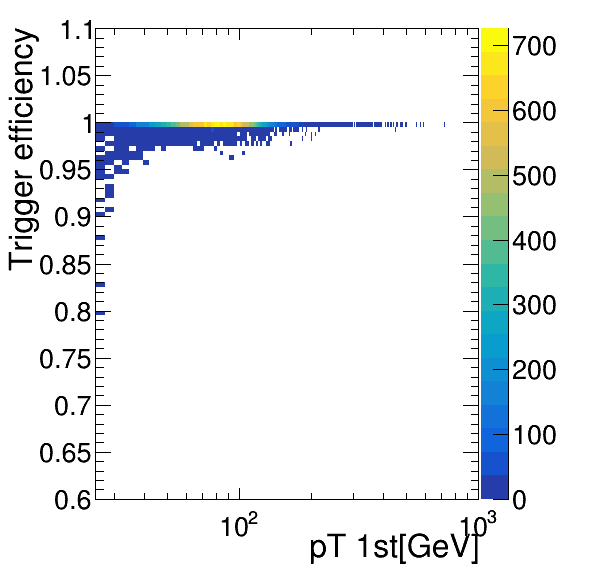
\includegraphics[width=0.45\textwidth]{Figs/Trigger/ele1.png} &
 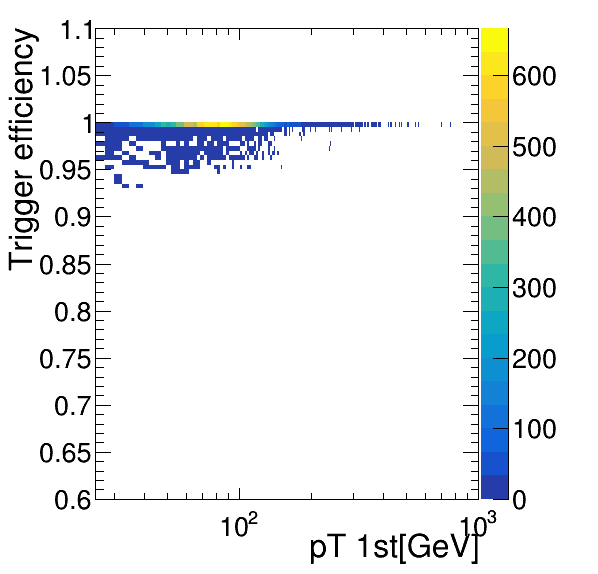
\includegraphics[width=0.45\textwidth]{Figs/Trigger/mu1.png} \\
 (a) electron 1st & (b) muon 1st \\
 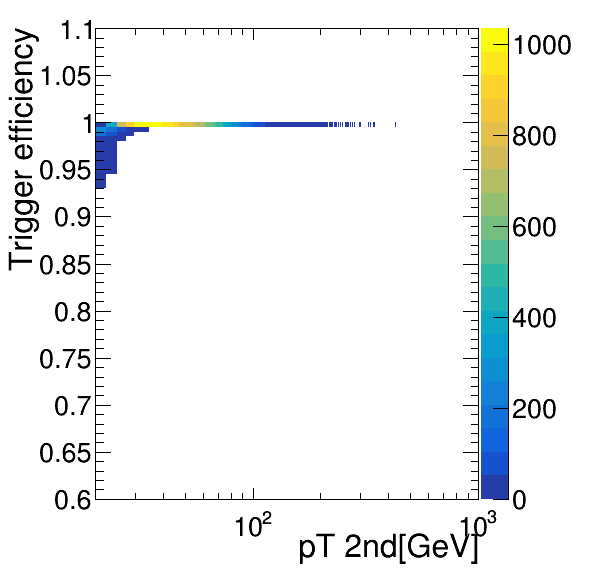
\includegraphics[width=0.45\textwidth]{Figs/Trigger/ele2.png} &
 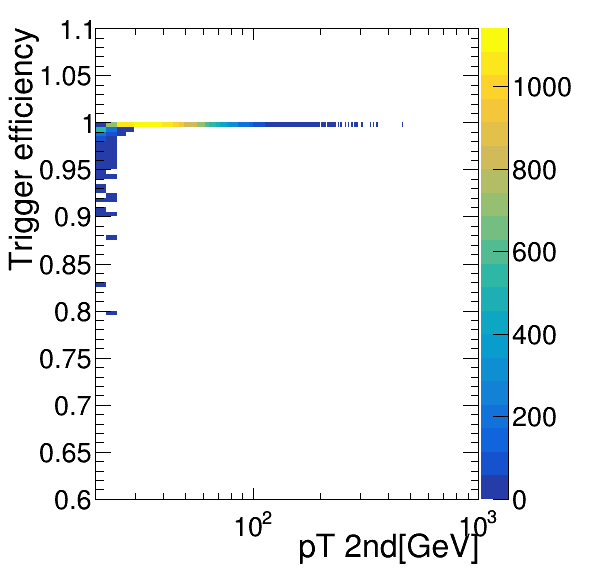
\includegraphics[width=0.45\textwidth]{Figs/Trigger/mu2.png} \\
 (c) electron 2nd & (d) muon 2nd \\
\end{tabular}
\caption{
      Trigger efficiency per event
      as a function of the lepton \pt
      for electrons (a) where leading lepton is an electron, 
      and (c) where trailing lepton is an electron, 
      and muons (b) where leading lepton is a muon, 
      and (d) where trailing lepton is an muon, 
      for a gluon fusion 300~\GeV MC sample.
      In this plots the other lepton not shown is
      integrated.
      An average trigger efficiency greater than 99\% is found.      
     }
    \label{Fig:trigger}
\end{figure*}

%  r99t /media/data/amassiro/LatinoTrees/Moriond/MCl2loose__hadd__bSFL2pTEff__l2tight/latino_GluGluHToWWTo2L2NuPowheg_M125.root
%  latino->Draw("effTrigW:std_vector_lepton_pt[0]","std_vector_lepton_pt[0]>10 && std_vector_lepton_pt[0]<50 && std_vector_lepton_pt[1]>13 && abs(std_vector_lepton_flavour[0]) == 11 && abs(std_vector_lepton_flavour[1]) == 13 ","colz")
%  latino->Draw("effTrigW:std_vector_lepton_pt[0]","std_vector_lepton_pt[0]>10 && std_vector_lepton_pt[0]<50 && std_vector_lepton_pt[1]>13 && abs(std_vector_lepton_flavour[0]) == 13 && abs(std_vector_lepton_flavour[1]) == 11 ","colz")
%     TH2F histo("histo","", 1000,20,100,   2000,0,1.1);
%     latino->Draw("effTrigW:std_vector_lepton_pt[0] >> histo","std_vector_lepton_pt[0]>20 && std_vector_lepton_pt[0]<100 && std_vector_lepton_pt[1]>10 && (abs(std_vector_lepton_flavour[1]) == 13 || std_vector_lepton_pt[1]>13) && abs(std_vector_lepton_flavour[0]) == 11 ", "colz");
%     latino->Draw("effTrigW:std_vector_lepton_pt[0] >> histo","std_vector_lepton_pt[0]>20 && std_vector_lepton_pt[0]<100 && std_vector_lepton_pt[1]>10 && (abs(std_vector_lepton_flavour[1]) == 13 || std_vector_lepton_pt[1]>13) && abs(std_vector_lepton_flavour[0]) == 13 ", "colz");
%     
%     TH2F histo("histo","", 1000,10,100,   2000,0,1.1);
%     latino->Draw("effTrigW:std_vector_lepton_pt[1] >> histo","std_vector_lepton_pt[0]>20 && std_vector_lepton_pt[1]<100 && std_vector_lepton_pt[1]>10 && (abs(std_vector_lepton_flavour[1]) == 13 || std_vector_lepton_pt[1]>13) && abs(std_vector_lepton_flavour[1]) == 11 ", "colz");
%     latino->Draw("effTrigW:std_vector_lepton_pt[1] >> histo","std_vector_lepton_pt[0]>20 && std_vector_lepton_pt[1]<100 && std_vector_lepton_pt[1]>10 && (abs(std_vector_lepton_flavour[1]) == 13 || std_vector_lepton_pt[1]>13) && abs(std_vector_lepton_flavour[1]) == 13 ", "colz");
%     
%     histo.GetXaxis()->SetTitle("p_{T} 1st [GeV]")
%     histo.GetYaxis()->SetTitle("Trigger Efficiency")
%     gPad->SetGrid();
%     histo.GetXaxis()->SetTitle("p_{T} 2nd [GeV]")




\begin{figure*}[htbp]
\centering
 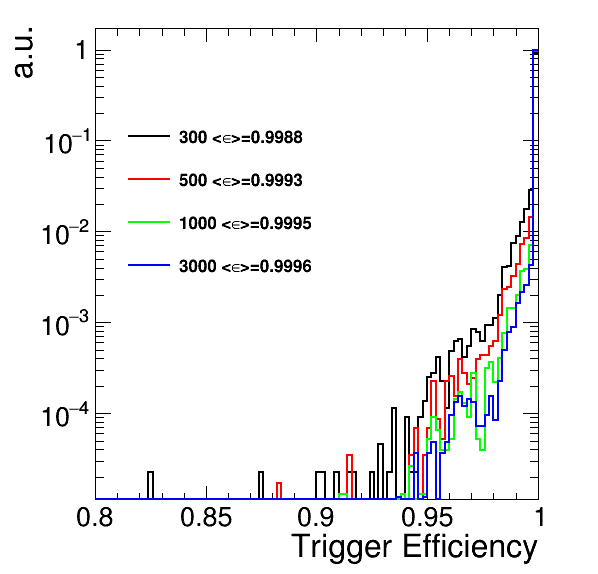
\includegraphics[width=0.45\textwidth]{Figs/Trigger/triggW.png}
\caption{
      Trigger efficiency distribution for 
      four MC samples corresponding to masses of 300, 500, 1000 and 3000~\GeV.
      An average trigger efficiency greater than 99\% is found.
     }
    \label{Fig:triggerIntegral}
\end{figure*}




The triggers used in the analysis are summarized in Table~\ref{tab:triggers} and 
described thoroughly in the separate analysis note, AN-17-082.



\subsection{MC samples}
%Monte Carlo
Concerning the simulated samples, several different Monte Carlo (MC) generators were used. 
In the simulation, `lepton' includes also $\tau$.
In order to perform the resonance search in a large part of the mass spectrum,
several signal samples for the gluon-gluon fusion and the vector boson fusion
mechanisms have been generated corresponding to different Higgs boson masses
in the range between 200\GeV and 3\TeV. The signal lineshape for each mass point corresponds to the one expected for a SM Higgs boson at that mass.
All signal samples, presented in Table~\ref{tab:signal}, have been simulated with
\POWHEG v2~\cite{Nason:2004rx,Frixione:2007vw,Alioli:2010xd}, designed to describe the full NLO properties of these processes.
In particular, for Higgs produced via gluon fusion~\cite{Alioli:2008tz}, and vector-boson-fusion (VBF)~\cite{Nason:2009ai},
the decay of the Higgs boson into two W boson and subsequently into leptons
was done using JHUGen v6.2.8~\cite{jhugen} for samples up to 300~\GeV of mass
and with v6.9.8 above that mass.
The signals which correspond to a Higgs boson mass of 125\GeV have been simulated accordingly and are treated as backgrounds in the analysis, including the associated production with a vector boson ($\mathrm{W^{+}H}$, $\mathrm{W^{-}H}$, ZH)~\cite{Luisoni:2013kna}, and gluon fusion produced ZH (ggZH). For associated production processes the Higgs boson decay was done via \PYTHIA 8.1~\cite{Sjostrand:2007gs}.


%
\begin{table*}[htbH]
\begin{center}
\small{
\begin{tabular}{@{}|l|c|c|@{}}
\hline
Process & Dataset Name & Number of events\\
\hline
\multirow{3}{*}{ggH} 			&  GluGluHToWWTo2L2Nu\_M125\_13TeV\_powheg\_JHUgen\_pythia8      &   500K \\	
					&  GluGluHToWWTo2L2Nu\_M200\_13TeV\_powheg\_JHUgenv628\_pythia8 &   100K \\
					&  GluGluHToWWTo2L2Nu\_M250\_13TeV\_powheg\_JHUgenv628\_pythia8 &   100K \\
					&  GluGluHToWWTo2L2Nu\_M300\_13TeV\_powheg\_JHUgenv698\_pythia8 &   100K \\
					&  GluGluHToWWTo2L2Nu\_M350\_13TeV\_powheg\_JHUgenv698\_pythia8 &   100K \\
					&  GluGluHToWWTo2L2Nu\_M400\_13TeV\_powheg\_JHUgenv698\_pythia8 &   100K \\
					&  GluGluHToWWTo2L2Nu\_M450\_13TeV\_powheg\_JHUgenv698\_pythia8 &   100K \\
					&  GluGluHToWWTo2L2Nu\_M500\_13TeV\_powheg\_JHUgenv698\_pythia8 &   100K \\
					&  GluGluHToWWTo2L2Nu\_M550\_13TeV\_powheg\_JHUgenv698\_pythia8 &   100K \\
					&  GluGluHToWWTo2L2Nu\_M600\_13TeV\_powheg\_JHUgenv698\_pythia8 &   100K \\
					&  GluGluHToWWTo2L2Nu\_M650\_13TeV\_powheg\_JHUgenv698\_pythia8 &   100K \\
					&  GluGluHToWWTo2L2Nu\_M700\_13TeV\_powheg\_JHUgenv698\_pythia8 &   100K \\
					&  GluGluHToWWTo2L2Nu\_M750\_13TeV\_powheg\_JHUgenv698\_pythia8 &   100K \\
					&  GluGluHToWWTo2L2Nu\_M800\_13TeV\_powheg\_JHUgenv698\_pythia8 &   100K \\
					&  GluGluHToWWTo2L2Nu\_M900\_13TeV\_powheg\_JHUgenv698\_pythia8 &   100K \\
					&  GluGluHToWWTo2L2Nu\_M1000\_13TeV\_powheg\_JHUgenv698\_pythia8 &   100K \\
					&  GluGluHToWWTo2L2Nu\_M1500\_13TeV\_powheg\_JHUgenv698\_pythia8 &   100K \\
					&  GluGluHToWWTo2L2Nu\_M2000\_13TeV\_powheg\_JHUgenv698\_pythia8 &   100K \\
					&  GluGluHToWWTo2L2Nu\_M2500\_13TeV\_powheg\_JHUgenv698\_pythia8 &   100K \\
					&  GluGluHToWWTo2L2Nu\_M3000\_13TeV\_powheg\_JHUgenv698\_pythia8 &   100K \\
					\hline
\multirow{3}{*}{VBF} 			&  VBFHToWWTo2L2Nu\_M125\_13TeV\_powheg\_JHUgen\_pythia8      &   500K \\	
					&  VBFHToWWTo2L2Nu\_M200\_13TeV\_powheg\_JHUgenv628\_pythia8 &   100K \\		
					&  VBFHToWWTo2L2Nu\_M250\_13TeV\_powheg\_JHUgenv628\_pythia8 &   100K \\
					&  VBFHToWWTo2L2Nu\_M300\_13TeV\_powheg\_JHUgenv698\_pythia8 &   100K \\
					&  VBFHToWWTo2L2Nu\_M350\_13TeV\_powheg\_JHUgenv698\_pythia8 &   100K \\
					&  VBFHToWWTo2L2Nu\_M400\_13TeV\_powheg\_JHUgenv698\_pythia8 &   100K \\
					&  VBFHToWWTo2L2Nu\_M450\_13TeV\_powheg\_JHUgenv698\_pythia8 &   100K \\
					&  VBFHToWWTo2L2Nu\_M500\_13TeV\_powheg\_JHUgenv698\_pythia8 &   100K \\
					&  VBFHToWWTo2L2Nu\_M550\_13TeV\_powheg\_JHUgenv698\_pythia8 &   100K \\
					&  VBFHToWWTo2L2Nu\_M600\_13TeV\_powheg\_JHUgenv698\_pythia8 &   100K \\
					&  VBFHToWWTo2L2Nu\_M650\_13TeV\_powheg\_JHUgenv698\_pythia8 &   100K \\
					&  VBFHToWWTo2L2Nu\_M700\_13TeV\_powheg\_JHUgenv698\_pythia8 &   100K \\
					&  VBFHToWWTo2L2Nu\_M750\_13TeV\_powheg\_JHUgenv698\_pythia8 &   100K \\
					&  VBFHToWWTo2L2Nu\_M800\_13TeV\_powheg\_JHUgenv698\_pythia8 &   100K \\
					&  VBFHToWWTo2L2Nu\_M900\_13TeV\_powheg\_JHUgenv698\_pythia8 &   100K \\
					&  VBFHToWWTo2L2Nu\_M1000\_13TeV\_powheg\_JHUgenv698\_pythia8 &   100K \\				
					&  VBFHToWWTo2L2Nu\_M1500\_13TeV\_powheg\_JHUgenv698\_pythia8 &   100K \\				
					&  VBFHToWWTo2L2Nu\_M2000\_13TeV\_powheg\_JHUgenv698\_pythia8 &   100K \\				
					&  VBFHToWWTo2L2Nu\_M2500\_13TeV\_powheg\_JHUgenv698\_pythia8 &   100K \\				
					&  VBFHToWWTo2L2Nu\_M3000\_13TeV\_powheg\_JHUgenv698\_pythia8 &   100K \\	\hline			
\end{tabular}
\caption{Reference signal samples used in the analysis. 
\label{tab:signal}}
\end{center}
}
\end{table*}
%

The \WW production, irreducible background for the analysis, was simulated in different ways. 
\POWHEG v2~\cite{Melia:2011tj} was used for \qqbar induced \WW in different decays. 
The cross section used for normalizing WW processes produced via \qqbar was computed at next-to-next-to-leading order (NNLO)~\cite{Gehrmann:2014fva}. 
In order to control the top quark background processes, the analysis is
performed in jet bins. The jet binning enhances the importance of logarithms of the jet \pt, spoiling the convergence of 
fixed-order calculations of the qq$\rightarrow$WW process and requiring the use of dedicated resummation techniques for an
accurate prediction of differential
distributions~\cite{Meade:2014fca,Jaiswal:2014yba}.  
Since the \pt of the jets produced in association with the WW system is strongly correlated with its transverse momentum, 
\pt$^{WW}$,  the simulated qq$\rightarrow$WW events are reweighted  
to reproduce the \pt$^{WW}$ distribution from the \pt-resummed calculation.

Gluon fusion produced \WW was generated, with and without Higgs diagrams, using \MCFM v7.0~\cite{Campbell:2013wga}. 
A \ttbar sample dilepton sample was also generated using \POWHEG v2. The \WW and \ttbar samples 
produced specifically for this analysis are presented in Table~\ref{tab:wwl}.


\begin{table*}[htbH]
\begin{center}
\footnotesize{
\begin{tabular}{@{}|l|c|c|c|@{}}
\hline
Process & Dataset Name & Events & $\sigma\times$BR [pb] \\
\hline
\ttbar$\rightarrow$\WW$b\bar{b}\rightarrow2l2\nu b\bar{b}$ & TTTo2L2Nu\_13TeV-powheg & 5M  & 87.31 \\
\hline
\qqbar$\rightarrow$\WW$\rightarrow2l2\nu$ & WWTo2L2Nu\_13TeV-powheg & 2M & 12.178 \\
 \qqbar$\rightarrow$\WW$\rightarrow l\nu qq$ & WpWmJJ-QCD-noTop\_13TeV-powheg &  & \\
% \qqbar$\rightarrow$\WW$\rightarrow4q$ & WWTo4Q\_13TeV-powheg & 2M & 51.723\\ \hline
$gg\rightarrow$\WW$\rightarrow2l2\nu$ & GluGluWWTo2L2Nu\_MCFM\_13TeV & 500K & 0.5905 \\
%$gg\rightarrow$\WW$\rightarrow2l2\nu$ (H diagr.) & GluGluWWTo2L2Nu\_HInt\_MCFM\_13TeV & 500K & 0.9544\\
\hline

\end{tabular}
}
\caption{Simulated samples for \ttbar and \WW production.}
\label{tab:wwl}}
\end{center}
\end{table*}

Other background samples are used, a list of the most relevant ones is presented in Table~\ref{tab:otherbck}.

\begin{table*}[htbH]
\begin{center}
\footnotesize{
\begin{tabular}{@{}|l|c|c|c|@{}}
\hline
Process & Dataset Name &  $\sigma\times$BR [pb] \\
\hline
Single top & ST\_tW\_top\_5f\_inclusiveDecays\_13TeV-powheg-pythia8\_TuneCUETP8M1 &   35.85  \\
		& ST\_tW\_antitop\_5f\_inclusiveDecays\_13TeV-powheg-pythia8\_TuneCUETP8M1 &   35.85  \\
\hline
Drell-Yan 	& DYJetsToTauTau\_ForcedMuEleDecay\_M-50\_TuneCUETP8M1\_13TeV-amcatnloFXFX-pythia8\_ext1 & 1867 \\
                & DYJetsToLL\_M-50\_TuneCUETP8M1\_13TeV-madgraphMLM-pythia8 &  6025.26  \\
                & DYJetsToLL\_M-50\_HT100to200\_TuneCUETP8M1\_13TeV-madgraphMLM-pythia8 &  147.4  \\
                & DYJetsToLL\_M-50\_HT200to400\_TuneCUETP8M1\_13TeV-madgraphMLM-pythia8 &  40.99  \\
                & DYJetsToLL\_M-50\_HT400to600\_TuneCUETP8M1\_13TeV-madgraphMLM-pythia8 &  5.678  \\
                & DYJetsToLL\_M-50\_HT600toInf\_TuneCUETP8M1\_13TeV-madgraphMLM-pythia8 &  2.198  \\
\hline
Multibosons 	& WZTo2L2Q\_13TeV\_amcatnloFXFX\_madspin\_pythia8 &  5.5950 \\
		& ZZTo2L2Q\_13TeV\_amcatnloFXFX\_madspin\_pythia8 &  3.2210 \\
		& WWZ\_TuneCUETP8M1\_13TeV-amcatnlo-pythia8  &  0.1651 \\
		& WZZ\_TuneCUETP8M1\_13TeV-amcatnlo-pythia8 &  0.05565 \\
\hline
\end{tabular}
}
\caption{Simulated samples for other backgrounds used in the analysis. 
\label{tab:otherbck}}
\end{center}
\end{table*}

For the Drell-Yan backgrounds we use two different sets of samples. For the
opposite flavore analysis (Sec~\ref{sec:OF}), selecting events with an
electron and a muon, a dedicated sample in which only the
$Z/\gamma^{*}\rightarrow{}\tau\tau\rightarrow{e\mu\nu\nu}$ decay is simulated.
For the same flavor analysis (Sec.~\ref{sec:SF}), in which pairs of electrons
or muons are selected, a soup of different HT binned DY samples is used. A
detailed study about this soup is given below in Sec.~\ref{sec:DY}.

All processes are generated using the NNPDF3.0~\cite{Ball:2013hta,Ball:2011uy} parton distribution functions (PDF) for NLO generators,
while the LO version of the same PDF is used for LO generators. All the event generators are interfaced 
to \PYTHIA 8.1~\cite{Sjostrand:2007gs} for the showering of
partons and hadronization, as well as including a simulation of the underlying event (UE) and multiple interaction (MPI)
based on the CUET8PM1 tune~\cite{Khachatryan:2015pea}. 
%
%To estimate the systematic uncertainties related to the choice of UE and MPI tune, the signal processes and the WW
%events are also generated with two alternative tunes which are representative of the errors on the tuning parameters.
%The showering and hadronization systematic uncertainty is estimated by interfacing the same MC samples with the 
%\HERWIG{}++ 2.7 parton shower~\cite{Richardson:2013nfo,Bellm:2013hwb}.
%

For all processes, the detector response is simulated using a detailed
description of the CMS detector, based on the \GEANT{}4 package~\cite{Agostinelli:2002hh}. 
The MC samples used  are part of the RunIISummer16MiniAODv2 campaign with the global tag:
\begin{center} \emph{PUMoriond17\_80X\_mcRun2\_asymptotic\_2016\_TrancheIV\_v6} \end{center}
and the CMSSW version used is \emph{8\_0\_26\_patch1}.

%PU
The simulated samples are generated with distributions for the number of pileup interactions that are meant to roughly cover,
though not exactly match, the conditions expected for the different data-taking periods. In order to factorize these effects, 
the number of true pileup interactions from the simulation truth (as stored in the PileupInfo collection in the Monte Carlo)
is reweighted to match the data.
The re-weighting is propagated automatically to both the in-time pile up and the out-of-time one.
In Figure~\ref{Fig:pu}, the effect of this reweighting on a sample enriched in Drell-Yan events is shown.
In order to select this sample, 
events with two electrons with \pt$> 25$~\GeV for the leading one and  \pt$>
13$~\GeV for the trailing one, are selected only if  $|\mll - m_Z| < 10$~\GeV. 

\begin{figure*}[htbp]
\centering
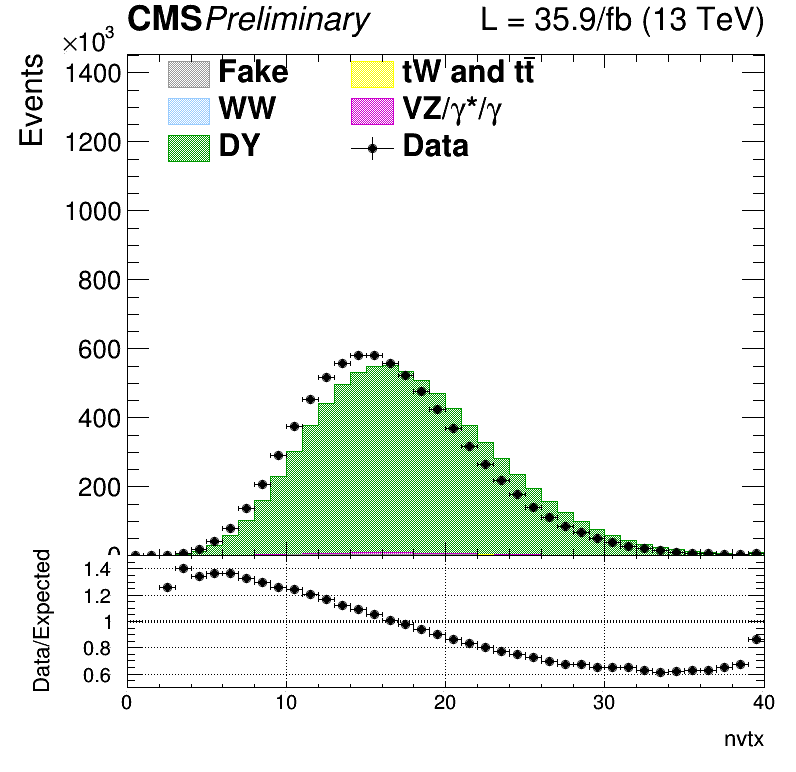
\includegraphics[width=0.45\textwidth]{Figs/nvertices.png}
\caption{
    Distributions of the number of vertices in a Drell-Yan enriched sample
    (Z$\rightarrow{}ee$) in
    data}
    \label{Fig:pu}
\end{figure*}

The pileup histogram for reweighting is calculated using the \emph{pileupCalc} tool as described in~\cite{puJSON}. 


%Cross sections
Different sources and calculations are used to obtain the cross sections for the different processes at 13\TeV. 
For Higgs signals, the cross sections used are the ones reported but the LHC Higgs Cross Section Working Group~\cite{temphiggsxsecs},
computed at NNLO and NNLL QCD and NLO EW for gluon fusion, and at NNLO QCD and NLO EW for the rest of the production modes.
The branching fractions are the ones reported in Ref.~\cite{Heinemeyer:2013tqa}. 

The cross section used for normalizing \qqbar produced WW processes was computed at next-to-next-to-leading order
(NNLO)~\cite{Gehrmann:2014fva}. The leading-order (LO) cross section for ggWW is obtained directly from \MCFM.
For gluon fusion, the difference between LO and NLO cross sections is significantly big.
A scale factor of 1.4 is theoretically calculated~\cite{Caola:2015rqy} and applied to the gg$\to$WW background. 
%The interference between the high mass resonance, the gg$\to$WW background and the H(125) has been computed using the MELA package as describe in Sec.~\ref{sec:AnalysisStrategy}.

%For the LO simulation of the interference between 
%gg$\rightarrow$WW and gluon fusion  produced H$\rightarrow$WW a k-factor of 1.87 is applied. 
%This k-factor is obtained as the average between LO to NNLO ggH scale factor and LO to NLO ggWW scale factor 
%(from private communication with the authors of~\cite{Caola:2015rqy}). 

The cross sections of the different single top processes are estimated by the LHC Top Working group~\cite{singletop} at NLO.
The \ttbar cross section is also provided by the LHC Top Working group~\cite{topxsec}, and it is computed at NNLO, with NNLL soft gluon resummation. 

Drell-Yan (DY) production of Z/$\gamma^{*}$ is generated using a\MADGRAPH~\cite{Alwall:2014hca} and the cross section is scaled using a LO to NNLO k-factor equal to 1.23. 
Other multiboson processes, such as WZ,ZZ, and VVV (V=W/Z), are generated with a\MCATNLO and normalized
to the cross section obtained at NLO in generation.
The cross sections for the remaining processes were directly obtained using the \emph{GenXSecAnalyzer}
tool~\cite{genxsec} or from the Twiki presented in Ref.~\cite{25nstwiki}.

All processes are generated using the NNPDF2.3~\cite{Ball:2013hta,Ball:2011uy} parton distribution functions (PDF) for NLO generators,
while the LO version of the same PDF is used for LO generators. All the event generators are interfaced 
to \PYTHIA 8.1 for the showering of partons and hadronization, as well as including a simulation of the 
underlying event (UE) and multiple interaction (MPI) based on the CUET8PM1 tune~\cite{Khachatryan:2015pea}.





\subsection{The DY sample}\label{sec:DY}

Given the lack of MC statistics in the LO inclusive DY sample the
$H_\mathrm{T}$-binned samples are used. This helps increasing the MC
statistics especially in the VBF category of the same flavor analysis, which is characterized by large values of $H_\mathrm{T}$.
The LO inclusive sample is used for events with $H_\mathrm{T} < 100$\GeV and it has been merged to the other samples selecting events with $H_\mathrm{T}$ below 100\GeV using the parton level information. The cross sections of those samples have been scaled applying the LO to NNLO k-factor. In Fig.~\ref{fig:DY_HT} the $H_\mathrm{T}$ distribution of the sample after the merging is reported, showing a smooth transition between different $H_\mathrm{T}$ samples.

\begin{figure}[htbp]
\centering
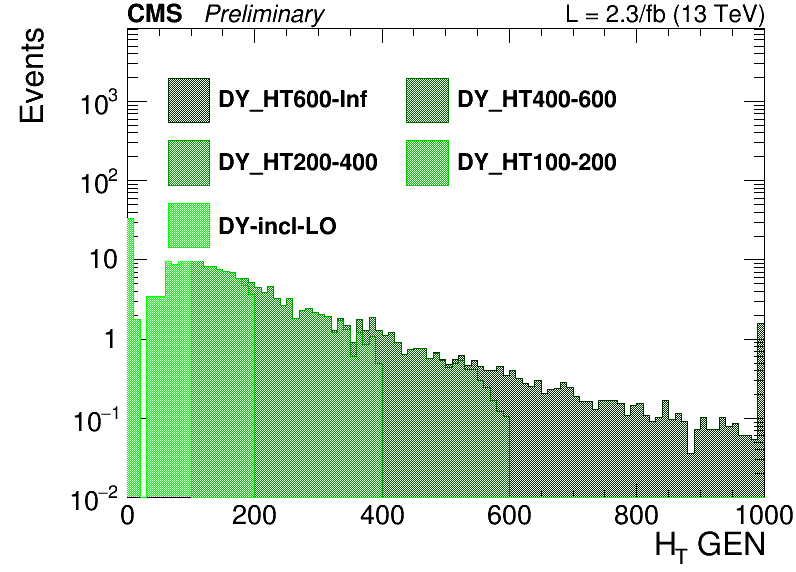
\includegraphics[width=0.6\textwidth]{Figs/log_c_incl_HTGen.png}
\caption{
    $H_\mathrm{T}$ distribution for the merged DY sample.}
    \label{fig:DY_HT}
\end{figure}


To further check the correct behaviour of the $H_\mathrm{T}$ binned samples we compared them to the inclusive LO sample, selecting only the events with a generator level $H_\mathrm{T}$ above 100\GeV. The comparison is done in a control region with two same flavor leptons with $\pt > 20$\GeV and $\mll > 50$\GeV, showing very good agreement between the two samples. The distributions of some variables are shown in Fig.~\ref{fig:inclDYvsHT}

\begin{figure}[htbp]
\centering
\subfigure[\mll]{
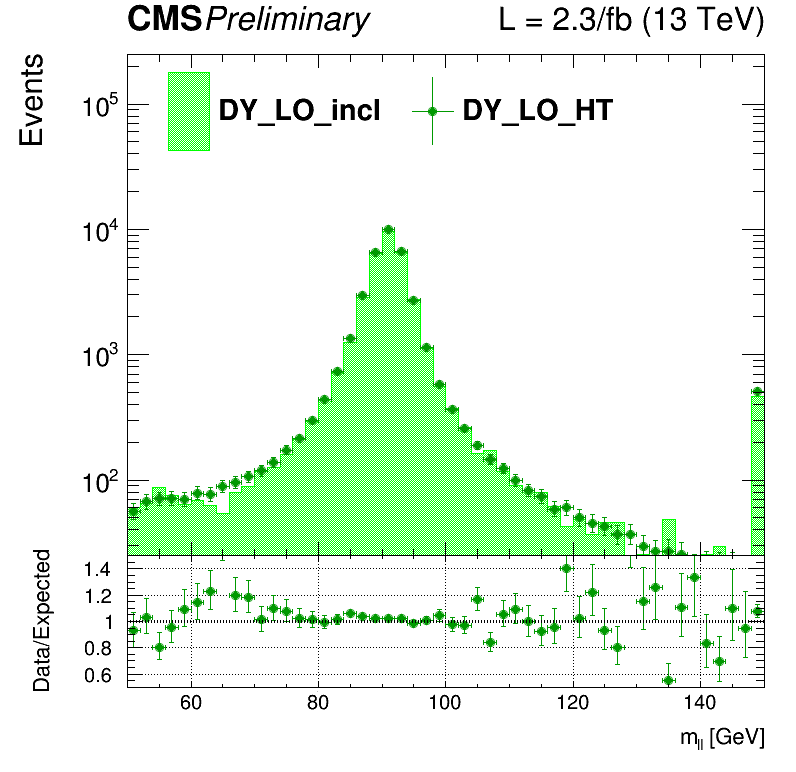
\includegraphics[width=0.45\textwidth]{Figs/DY/inclLOvsHT/log_cratio_dyee_13TeV_mll.png}
}
\subfigure[\ptll]{
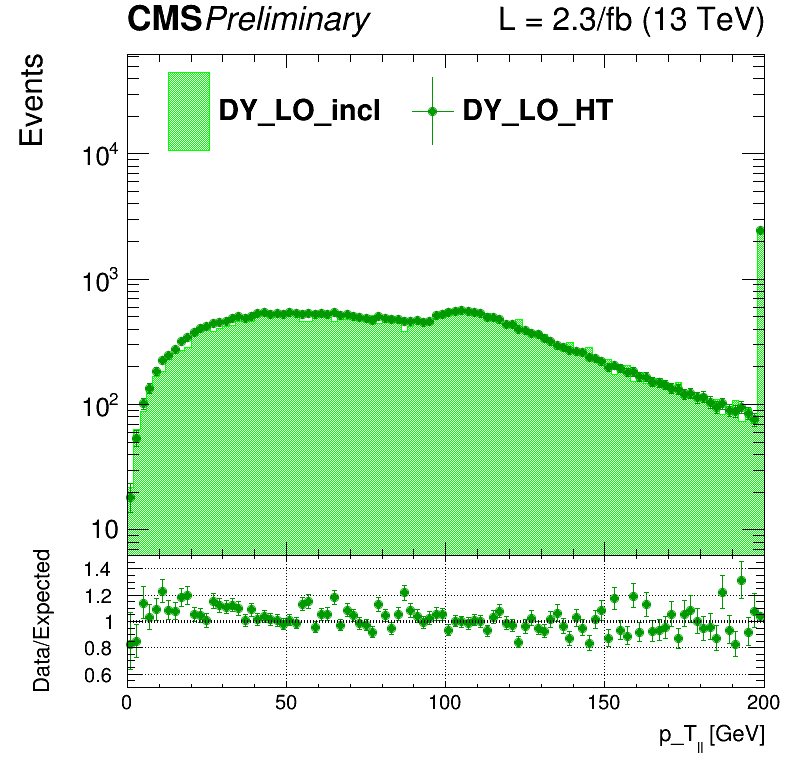
\includegraphics[width=0.45\textwidth]{Figs/DY/inclLOvsHT/log_cratio_dyee_13TeV_ptll.png}
}
\\
\subfigure[$\eta$ of leading lepton]{
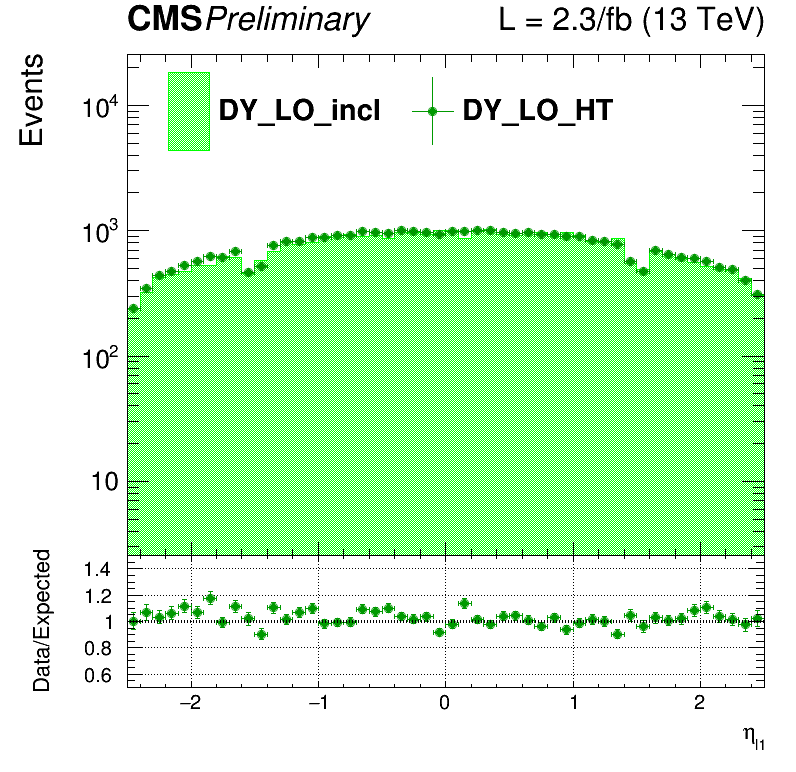
\includegraphics[width=0.45\textwidth]{Figs/DY/inclLOvsHT/log_cratio_dyee_13TeV_eta1.png}
}
\subfigure[$\eta$ of trailing lepton]{
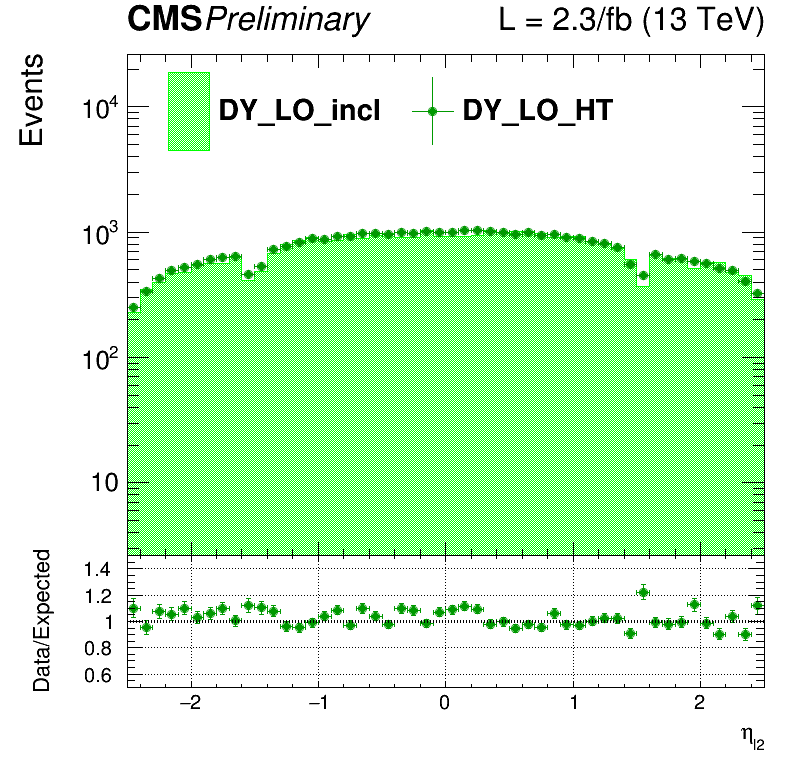
\includegraphics[width=0.45\textwidth]{Figs/DY/inclLOvsHT/log_cratio_dyee_13TeV_eta2.png}
}
\caption{
    Comparison between the inclusive LO DY sample and the $H_\mathrm{T}$ binned samples.}
    \label{fig:inclDYvsHT}
\end{figure}



To check the differences between the LO inclusive sample and the NLO sample simulated with \MCATNLO, the two samples have been compared in a same flavor control region and some variables of interest are shown in Fig.~\ref{fig:LOvsNLO}. The control region is defined requiring two same flavor leptons with $\pt > 20$\GeV and with $\mll > 50$\GeV.


\begin{figure}[htbp]
\centering
\subfigure[\mll]{
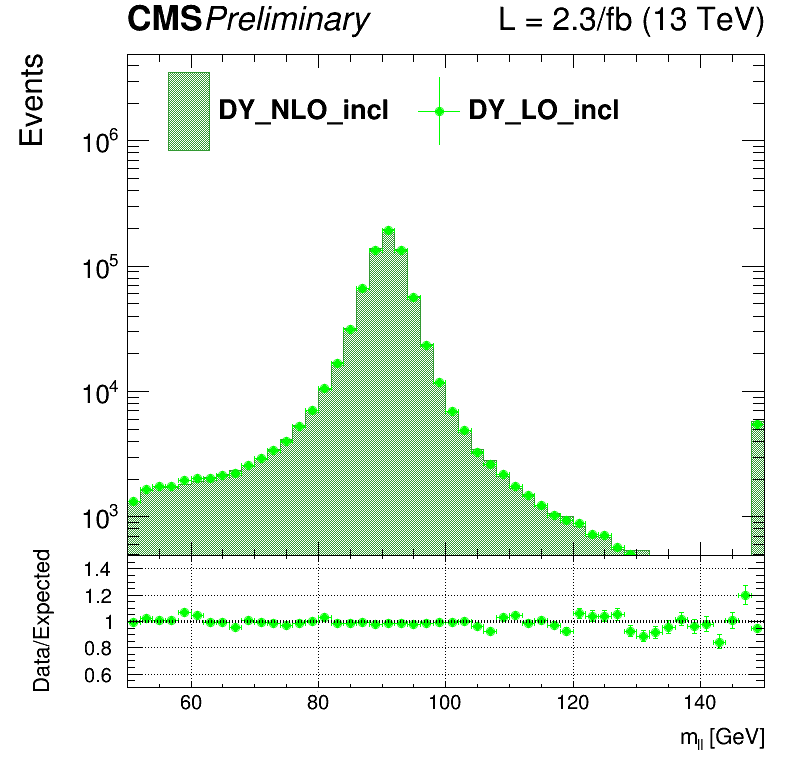
\includegraphics[width=0.45\textwidth]{Figs/DY/LOvsNLO/log_cratio_dyee_13TeV_mll.png}
}
\subfigure[\ptll]{
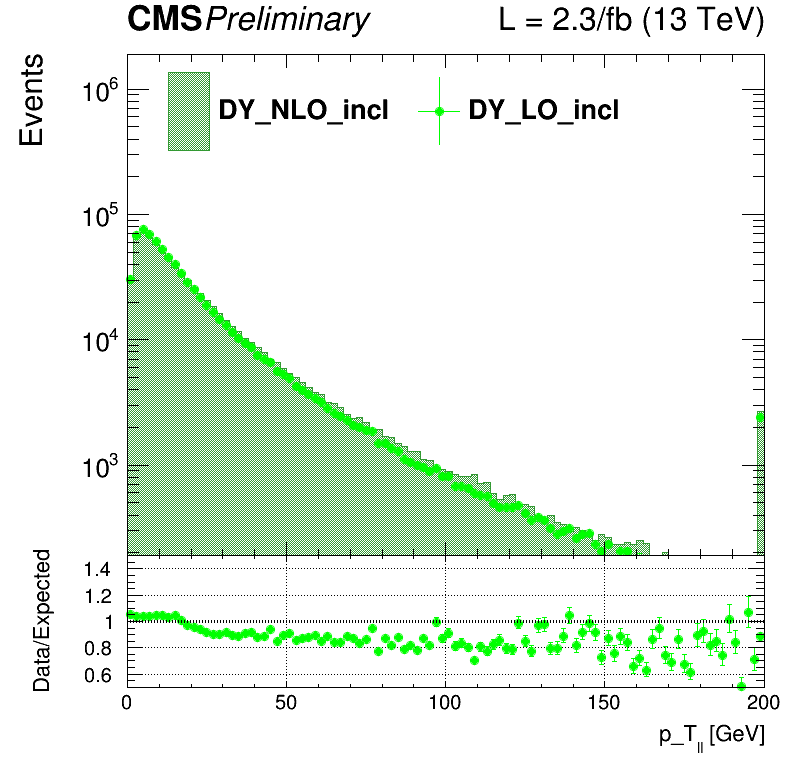
\includegraphics[width=0.45\textwidth]{Figs/DY/LOvsNLO/log_cratio_dyee_13TeV_ptll.png}
}
\\
\subfigure[$\eta$ of first lepton]{
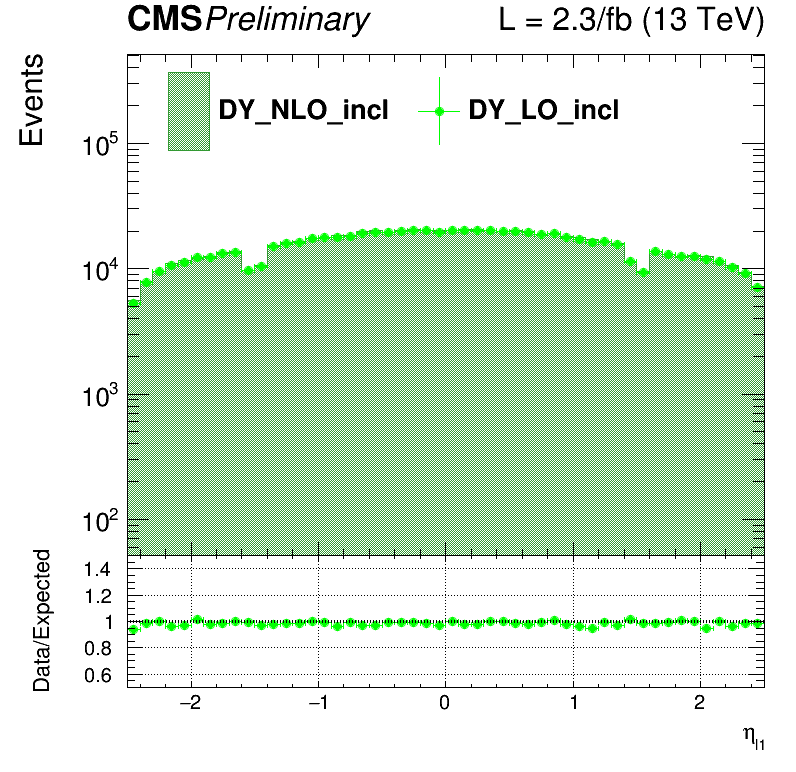
\includegraphics[width=0.45\textwidth]{Figs/DY/LOvsNLO/log_cratio_dyee_13TeV_eta1.png}
}
\subfigure[number of jets]{
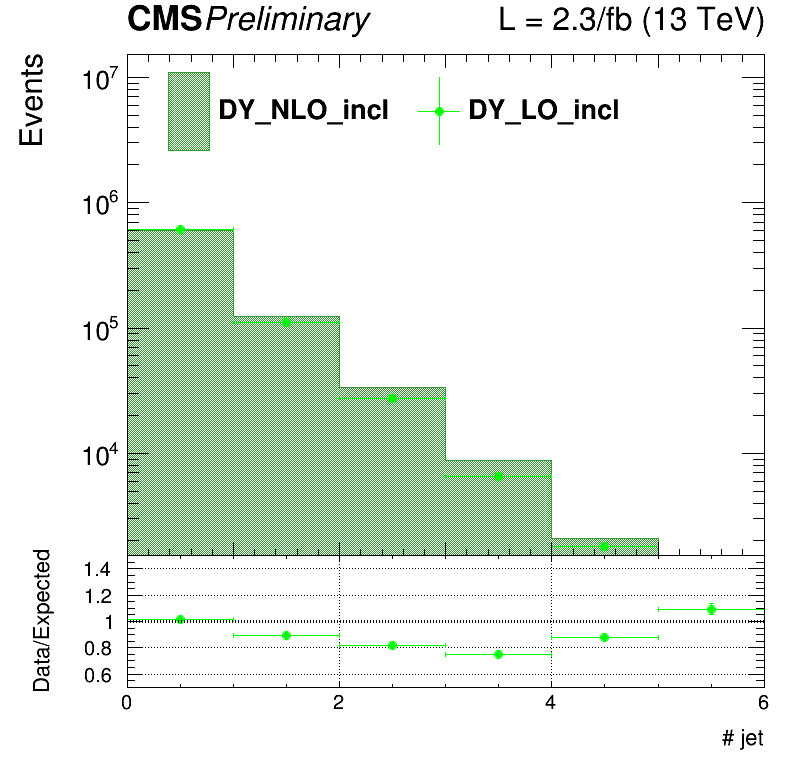
\includegraphics[width=0.45\textwidth]{Figs/DY/LOvsNLO/log_cratio_dyee_13TeV_njet.png}
}
\caption{
    Comparison between the LO and NLO DY samples.}
    \label{fig:LOvsNLO}
\end{figure}


\subsection{The WW sample}

In the analysis two different WW Monte Carlo samples are merge: the ``$WW \rightarrow 2l 2\nu$ NLO'' and the ``WW plus 2 jet'' LO (WpWmJJ-QCD-noTop in Tab. 4). 

The second sample,  ``WW plus 2 quark'', contais final state with two quarks or a gluon-quark system: only the final state with two quarks interferes with the signal.
To avoid double count between the two sample a cut on di-jet mass at gen-level,$mjj_{GenLev}$, is applied. In particular the sample ``$WW \rightarrow 2l 2\nu$ at NLO'' is used for $mjj_{GenLev} <100$ GeV and the ``WW plus 2 quark'' for $mjj_{GenLev} >100$ GeV.

The  distribution for the reco di-jet mass is shown in Fig. \ref{fig:WW}. In particular the red distribution correspond the ``$WW \rightarrow 2l 2\nu$ NLO'' sample with a cut of  $mjj_{GenLev} <100$, the blue distribution to  ``WW plus 2 quark'' with $mjj_{GenLev} >100$ GeV. The sum of the red and blue distributions is shown in black. There is a good agreement between with the black distribution and the ``$WW \rightarrow 2l 2\nu$ NLO'' without any  $mjj_{GenLev}$ distribution , in green.



\begin{figure}[htbp]
\centering
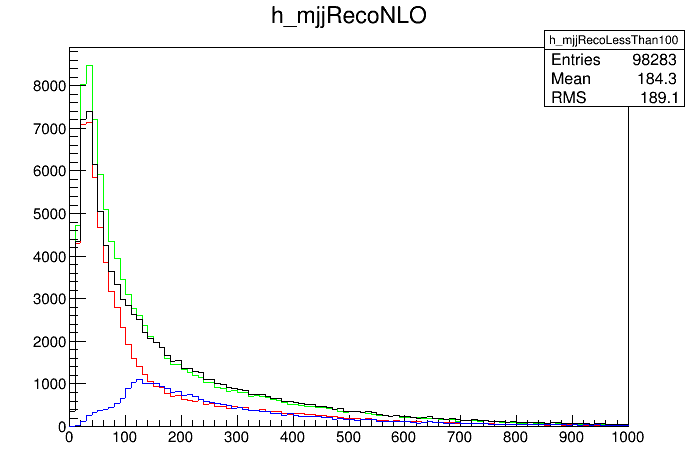
\includegraphics[width=0.6\textwidth]{Figs/WW_distribution.png}
\caption{
    Distribution for $m_{jj}$ at RECO level for the merged WW sample.}
    \label{fig:WW}
\end{figure}

